%%%%%%%%%%%%%%%%%%%%%%%%%%%%%%%%%%%%%%%%%%%%%%%%%%%%%%%%%%%%%%%%%%%%%%%%%%%%%%%
%                                                                             %
% Cette version repart de 03_Draft\appendix\appendix_negotiations_current.tex %
%                                                                             %
%%%%%%%%%%%%%%%%%%%%%%%%%%%%%%%%%%%%%%%%%%%%%%%%%%%%%%%%%%%%%%%%%%%%%%%%%%%%%%%

In section \ref{sec:Nego} of the paper, we investigate the link between displacement and change in firm-level negotiations characteristics, making use of two administrative data sets that provide firm-level characteristics relative to workplace negotiations. We provide more detail on the data used. The first data gives detailed information about collective agreements signed (or discussed) within firms. The second data measures turnout and results from workplace elections. These two data sets provide rare and direct insight into in-house bargaining, a potential mechanism underlying the loss in firm-level wage premia experienced by displaced workers. In this online appendix section, we first present the collective agreements data in subsection \ref{appsec:accord_data} and the election data in subsection \ref{appsec:elec_data}. In subsection \ref{appsec:robust_samples} we show that the sample restrictions we make for this analysis do not affect our main conclusions. Finally, in subsection \ref{appsec:neg:results} we display more detailed results, complementing the analysis presented in the main text. 

\subsection{Collective agreements\label{appsec:accord_data}}

% https://www.service-public.fr/professionnels-entreprises/vosdroits/F31400

In order to document the number and type of collective agreements signed by firms, we use the ``D@ccord'' data set, produced by the Ministry of Labor research and statistics direction (DARES), and available since 2005. The French labor law requires firm-level collective agreements to be filed on a dedicated online platform. Each negotiation has to be reported, even when no agreement is reached. The D@ccord data contains information on the type of reported text, be it an actual firm-level collective agreement, or a report of disagreement. It also provides information on the matter of the negotiations (e.g. wages, hours, layoffs, etc.), on the parties negotiating or signing the agreement, the date of signature of the agreement, and the firm identifier (SIREN), which we use to match this data with our main samples (LE or MLO).

The D@ccord data enables us to build several variables describing the type, number and subject of collective agreements signed each year in a given firm. We consider 3 main bargaining subjects: agreements on wages and bonuses; agreements related to earnings more generally (wages and bonuses, ranking,\footnote{Within a firm, a worker's ranking (\textit{classification} in French) is used to determine the position, duties and minimum wage applicable to the employee.} profit-sharing and participation); agreements related to hours and working time.

Our main measure of collective agreement is an indicator taking value 1 if a firm has signed (at least) one agreement relative to earnings (i.e. type 1.) over the 2005-2007 period, and 0 otherwise. We assign 0 to firm for which we do not observe any agreements (our results are robust to excluding those) -> (\textcolor{red}{this is the old definition, we have the that the firm has to have operated during 2005-2007 and has at least 50 workers}) \textcolor{orange}{[proposed: ``The sample is restricted to firms that operated over 2005--2007 and had at least 50 employees; firms for which no agreement is observed are assigned 0 (our results are robust to excluding them).'']}. Alternatively, we consider a continuous version of the outcome, summing all the observed agreements on earnings over the period (and assigning 0 to other firms). Next, we consider failed negotiations about the same topic; that is negotiations that yield no signed agreement. Finally, we also consider indicators for the signature of (at least) one agreement of each of the other types separately. 

Table \ref{tab:nego:LEnego_acc_desc} describes the distribution of those outcomes in our sample of analysis. About 61.5\% of firms employing individuals in our sample \textcolor{orange}{[24.6\%: Table~\ref{tab:nego:LEnego_acc_desc}, mean 0.246]} have signed (at least) one agreement about wages over 2005-2007. This leads to an average number of 2.27 agreements \textcolor{orange}{[0.89]} signed by those firms over the period. At the same time, 26.9\% also failed to sign \textcolor{orange}{[10.4\%]} a wage agreement they had started to negotiate. Finally, 53.2\% signed an agreement on working time and hours \textcolor{orange}{[21.1\%]}.


% Est-ce qu'on dit participation en anglais ? ou les 2 (participation et intéressement) vont dans "profit sharing" ?

% L'intéressement est un dispositif d'épargne salariale lié aux résultats ou aux performances de l'entreprise. Toutes les entreprises peuvent le mettre en place, par voie d'accord avec les salariés. Le bénéficiaire de l'intéressement perçoit une prime dont le montant et les conditions de versement sont fixés par l'accord d'entreprise. Les sommes sont immédiatement disponibles, mais le salarié peut choisir de les placer sur un plan d'épargne salariale ou un compte épargne-temps.

% La participation est un mécanisme de redistribution des bénéfices de l'entreprise aux salariés. Elle est obligatoire dans les entreprises dont l'effectif est de 50 salariés ou plus. Le salarié bénéficiaire reçoit une prime dont le montant est fixé par l'accord de participation. Il peut demander le versement immédiat des sommes ou leur placement en épargne. Dans ce cas, les sommes sont indisponibles pendant 5 ans. L'accord de participation précise comment les sommes sont placées.

% 1. Salaires et primes (OBJN1)
% 2. Salaires et primes (OBJN1), Classifications (OBJN2), Intéressement (OBJN3), Participation (OBJN4)
% 3. Accords de méthode (PSE) (OBJN15), Accès et maintien des salariés dans l'emploi (OBJN16)
% 4. Durée collective temps de travail (anciennement RTT) (OBJN9), Aménagement du temps de travail (OBJN10), CET (OBJN11), Fixation des congés (anciennement "modulation") (OBJN11), Heures supplémentaires (OBJN34), Travail du dimanche (OBJN36)


\begin{table}[h]
\caption{Collective agreements outcomes, descriptive statistics}
\begin{center}
\label{tab:nego:LEnego_acc_desc}
\begin{adjustbox}{max width=\linewidth}
\begin{tabular}{l|lllllll}\toprule
% Generated from current results_analysis CSV files by master.R, section I (scripts/I-PLOTS_AND_TABLES).
% Table A16; status: ready
% Sample: le5_panelsize0-acco_alt. N counts nonmissing observations for each outcome; the treated count describes the full sample. Agreement outcomes cover 2005-2007; uses exported p75.
% -- means a requested statistic is unavailable; an empty cell means not applicable.
 & Mean & sd & min & p75 & max & $N$ \\
\hline
Wage agreement indicator & 0.541 & 0.498 & 0 & 1 & 1 & 90,120 \\
\# Wage agreement & 1.984 & 3.541 & 0 & 3 & 52 & 90,120 \\
Wage failure ind. & 0.232 & 0.422 & 0 & 0 & 1 & 90,120 \\
Hours agreement ind. & 0.466 & 0.499 & 0 & 1 & 1 & 90,120 \\
\hline
\# Treated (sample) & 16,512 &  &  &  &  &  \\

\bottomrule
\end{tabular}
\end{adjustbox}
\floatfoot{{\footnotesize \textsc{Notes}: This table provides simple descriptive statistics about collective agreements outcomes. \textbf{Sample}: The sample of interest is all workers laid-off for economic reason (LE) after 2007, and their respective controls. \textbf{Outcomes}: Table \ref{apptab:definitions} summarizes variables' definition. Wage agreement indicator takes value 1 if the firm has signed (at least) one agreement relative to wages, and 0 otherwise. \# Wage agreement is the number of wages agreement signed by the firm. Wage failure indicator takes value 1 if the firm has failed to conclude (at least) one negotiation relative to wages. Hours agreement indicator takes value 1 if the firm has signed (at least) one agreement relative to hours and working time.}}

\end{center}
\end{table}



% SAMPLE RESTRICTION
We use the collective agreements outcome to explore the evolution of firm-level characteristics (relative to negotiation) for displaced workers. Because the data starts in 2005 (i.e. after the first layoff we observe), one may worry about potential reverse causality. This would be the case if firm-level negotiations happen right after a layoff and respond to it. To limit this risk as much as possible, we focus our analysis on a sub-sample of displaced workers for which we can measure firm-level negotiations strictly before the layoff. In practice, we only consider workers affected by a layoff after 2007 while, at the same time, we construct firm outcomes over the 2005-2007 period only. In subsection \ref{appsec:robust_samples} below, we show that this sub-sample resembles our main sample of analysis and that our main results hold true.



 


\FloatBarrier
\subsection{Workplace elections\label{appsec:elec_data}}
We next observe workplace elections. Our data covers the 2009 to 2012 period and provides detailed measures on many elections (number of electors, number of voters, results by trade union, etc.). Workplace elections in France are very heterogeneous. This is because, within a common legal framework, each firm can set the exact format of its elections. Below, we briefly detail the main legal framework as well as the data we observe. In a nutshell, we use a firm-level measure of turnout at the elections as an indication of within-firm quality of negotiations.


\paragraph{Main legal framework}
In France (and over the period of interest), workers elect representatives at most every 4 years. Those representatives are elected for three distinct (but complementary) bodies:
\begin{itemize}
\item[-] The DP (for ``Délégué du Personnel'') in firms with 11 employees or more.

\item[-] The CE (for ``Comité d'Entreprise'') in firms with 50 employees or more. In those firms, CE and DP elections take place at the same time. Elected representatives can be member of the two bodies at the same time.

\item[-] The DUP (for ``Délégué Unique du Personnel'') can be elected in firms with 50 to 299 employees. They are meant to ease the negotiation by merging the three main bodies of workers' representation (the aforementioned DP and CE, and the ``CHSCT'' a third committee in charge of health and safety and whose member are designated by DP or CE).
\end{itemize}


\paragraph{Elections in practice}
%In practice, elections take place in a $Year \times Body \times Level \times Occupation$ stratum. The $Year$ is at most every four years, but partial elections can be organized if needed (i.e. when a representative and her substitute have to be replaced). The $Body$ is either DP, CE and/or DUP. The $Level$ can be either the firm or each establishment. And the $Occupation$ means that different occupations (e.g. blue collars, technicians or high-skilled professionals) can organize distinct elections. The exact stratum is actually defined differently in each firm, through internal negotiations prior to the election. To keep the simplest information here we: i) ignore partial elections and ii) aggregate the data at the firm level (weighting each $Body \times Level \times Occupation$ by its number of electors, when needed). That allows us to obtain one observation per firm, (at most) every 4 years. 

Within this main framework, each firm has the ability to decide about how the election is to be organized in practice. That is, prior to an election, within-firm negotiation will decide about strata in which (sub-)elections are organized. The choices relate to:
\begin{itemize}
\item[-] The body $b$ of the election. As explained before, depending on firm size, elections may take place to elect either DP and/or CE and/or DUP.
\item[-] The year $y$ of the election. Although every 4 years is legally binding, some firm may have to organize elections more often due to sector agreements or because a representative (and her substitute) has to be replaced in a partial elections. In our analysis, we ignore partial elections.\footnote{Election can have more than one round, but we focus our analysis on first round only. This is because the second round only takes place when the election fails either because i) no trade union ran for the election or ii) less than 50\% of electors voted. As explained below, we do take into account this type of failure.}
\item[-] The level $l$ which can be either the entire firm or its establishment separately.
\item[-] The occupation $o$ meaning that different types of workers (e.g. blue collars, engineers, etc.) can decide to vote in distinct elections.
\end{itemize}

Importantly, each firm will decide of a stratum defined by $b \times y \times l \times o$. For instance, one firm may have only one single election for all its workers (regardless of their establishments and occupation) to elect representative in DP and CE body; whereas another firm may organize election at the establishment-level, with each establishment following its own calendar (e.g. 2009-2013 for one, 2010-2014 for another, etc.). Given the number of possible options, there is substantial heterogeneity in size and timing of elections.

\paragraph{Data cleaning and outcomes definition} To ease the analysis, we collapse each election result at the firm times body (i.e. DP, CE, or DUP -- $b$) level. That is, we ignore the divisions in $l$, $o$ and $y$. Summing numbers across $l$ and $o$ is straightforward as those categories are exclusive (i.e. one worker belongs to one single establishment  and one single occupation). We decide to ignore years $y$ for two reasons. First because our data does not allow us to know whether different years simply reflect internal organization of the election (e.g. different establishments voting on different dates) or occurrence of main elections at less than 4 years interval. Second, over the 2009-2012 period, most firms (80\%) are observed in only 1 year. To aggregate information at the firm times body level, we weight each stratum by its number of electors. 

This simplification allows us to construct three main outcomes. First, we observe the average election turnout for the observed firms over the 2009-2012 period. This outcome is the average participation across the different bodies $b$ (i.e. between 1 and 3 distinct elections) of a given firm. We complement this main outcome with two others. The second outcome we compute is the share of workers who are covered by an election that failed;\footnote{An election fails if no trade union ran for the election.} where we think of election failure as an indication of a low quality of workplace negotiation. Finally, our third outcome is the share of workers who are covered by an election where a CGT representative received more than 10\% of the votes;\footnote{The 10\% threshold is important as it allows a candidate to become ``Délégué Syndicale'' or DS -- not DP --, who take part in negotiations about wages. This threshold is measured in the first round of the election.} where we think of CGT as indicating more conflictual negotiation. The CGT is one of the oldest (1895) and main trade union in France, traditionally seen as left-oriented (with marxist origins). A small literature also finds CGT union to be associated with higher wages \citep{abowd_persistent_2012, breda_firms_2015}. This renders the meaning of the CGT outcome more complex and suggests cautious interpration.

Table \ref{tab:nego:LEnego_ele_desc} describes the empirical distribution of those outcomes in the firms of our sample of analysis (cf. below about the sample). The workers in our sample are employed by firms that had an average turnout of 64.3\% \textcolor{orange}{[59.6\%: Table~\ref{tab:nego:LEnego_ele_desc}, mean 0.596]} at professional elections held over 2009-2012. On average in those firms, about 11.6\% of the workers were affected by failed election \textcolor{orange}{[22.4\%]}. Finally, about 50\% of the workers \textcolor{orange}{[OK: 50.4\%]} were involved in an election where a CGT candidate had received 10\% or more of the votes.

%A propos de 

%\iffalse 

%\begin{table}[h] 
%\caption{Elections sample}
%\begin{center}
%\input{03_Draft/tables/desc_nego_LE_elections.tex}  %\label{tab:nego:desc_nego_LE_elections}
%\floatfoot{{\footnotesize \textsc{Notes}: ...}} 
%\end{center}
%\end{table}

%\fi

%We are mainly interested in two dimensions of the election outcome: the turnout, and the vote for CGT. We consider turnout as an indicator of work relations within the firm. We next build an indicator taking the value 1 if the CGT union had a candidate in the election, and 0 otherwise. CGT is one of the oldest and most important Union in France (???) but is often regarded as more conflictual (???, SOURCE?). We view the presence of CGT as an indicator of ???.



\begin{table}[h]
	\caption{Elections outcomes, descriptive statistics}
	\begin{center}
		\label{tab:nego:LEnego_ele_desc}
		\begin{adjustbox}{max width=\linewidth}
\begin{tabular}{l|lllllll}\toprule
			% Generated from current results_analysis CSV files by master.R, section I (scripts/I-PLOTS_AND_TABLES).
% Table A17; status: ready
% Sample: le5_panelsize0-election. N counts nonmissing observations for each outcome; the treated count describes the full sample. Election outcomes cover 2009-2012; uses exported p50. Failed = no-candidate share, not blank votes.
% -- means a requested statistic is unavailable; an empty cell means not applicable.
 & Mean & sd & min & p50 & max & $N$ \\
\hline
Average turnout & 0.610 & 0.262 & 0 & 0.695 & 1.000 & 90,252 \\
Failed (\% workers) & 0.200 & 0.377 & 0 & 0.000 & 1.000 & 104,412 \\
CGT (\% workers) & 0.515 & 0.391 & 0 & 0.622 & 1.000 & 94,442 \\
\hline
\# Treated (sample) & 17,071 &  &  &  &  &  \\

			\bottomrule
		\end{tabular}
\end{adjustbox}
		

		\floatfoot{{\footnotesize \textsc{Notes}: This table provides simple descriptive statistics about professional election outcomes. \textbf{Sample}: The sample of interest is all workers laid-off for economic reason (LE), and their respective controls, whose firm have at least one election between 2009-2012 (observed in the data). \textbf{Outcomes}: Table \ref{apptab:definitions} summarizes variables' definition. Average turnout is the worker-weighted average participation of electors in firm-specific professional elections. See details in \ref{appsec:elec_data}. Failed is the share of firm's workers who were electors for a (eventually) failed election (i.e. no trade union ran). CGT is the share of firm's workers who were electors in an election were a CGT representative received more than 10\% of the votes.}} 
	\end{center}
\end{table}



Our data of workplace elections covers the end of our period of analysis (2009-2012). This timing is problematic because the majority of the layoffs we observe take place before. To limit the risk of reverse causality, we take advantage of our LE setting, where small (even individual) layoffs can be observed. In particular, we verify that our election results are robust to considering only a sub-sample of layoffs were the number of displaced workers is small, relative to the firm size. In our sample, this means considering layoffs affecting 6.7\% (\textcolor{red}{where does the number come from? to be removed}) \textcolor{orange}{[agreed: the 6.7\% cannot be traced to any table; drop it]} of firms' employees or less (the lowest 25\% in our sample -> \textcolor{red}{lowest quartile of the observed layoff-share measure in the election sample}).%\footnote{In the sample, 25\% of LE workers are observed along 0.56\% of their own firm' workforce. Given that we observe a 1/12 sample of workers, this represent about 6.7\% of firm's employees.}
 This robustness test addresses the risk that the relative decline in employers' average turnout result from an actual increase in previous employers' turnout (e.g. if workers vote more after a lay-off affected their colleagues) than a re-employment mechanism.



\FloatBarrier
\subsection{Robustness of the main results \label{appsec:robust_samples}}
The sample we use to perform analysis on collective agreements and elections differ from our main sample of analysis. In the case of collective agreements, this is because we consider only those workers who lost their job from 2008. In the case of electoral results, this is because we do not observe the universe of firms. Although we tried to follow transparent rules, nothing entirely prevents the selection of specific sub-samples. In this subsection, we show that these selections do not alter the sample observable characteristics too much and that our main results on labor (earnings, hours worked, wage rates and premia) %and firm (productivity, value added per worker, labor share, size) 
holds across samples.

Figure \ref{fig:neg:roblabor} below reproduce Figure \ref{fig:fe_current_event_mlo_pretrends} for the two sample we use when estimating effects in accords and elections outcomes. 

%XXX TO BE COMPLETED, GRAPHS READY: LE\_accords\_age\_robfirm \\
%or LE\_elections\_lnsize\_roblabor, etc.


\begin{figure}[h!] \centering
	\caption{Loss in wage premia for accords and election samples} \label{fig:neg:roblabor}
	\begin{subfigure}[b]{\textwidth}
		\centering
		\caption[]{\small Accords sample \label{fig:neg:roblabor:acc}}
		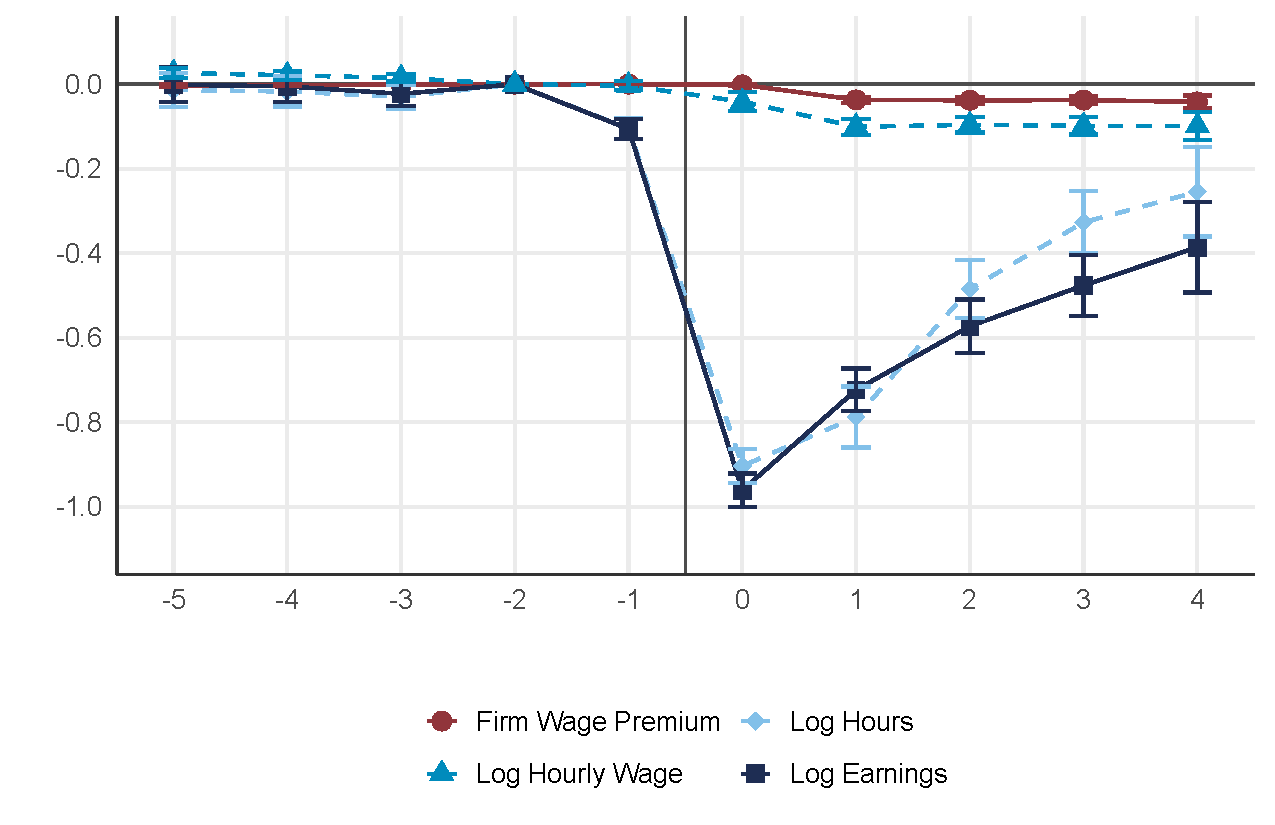
\includegraphics[width=.79\linewidth,max width=.79\linewidth]{figures/01_event_figures/figure_A20_a_agreements_sample.pdf}
	\end{subfigure}

	\begin{subfigure}[b]{\textwidth}
		\centering
		\caption[]{\small Election sample \label{fig:neg:roblabor:elec}}
		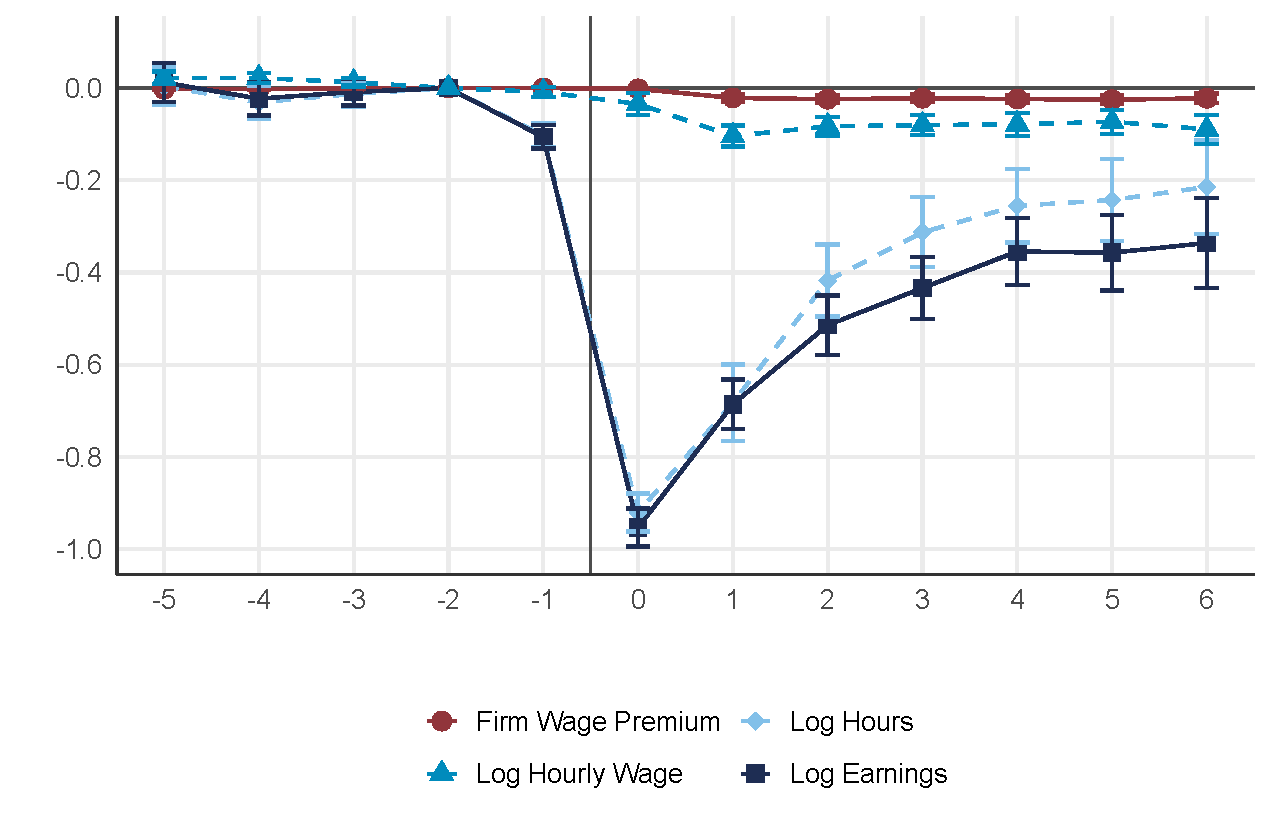
\includegraphics[width=.79\linewidth,max width=.79\linewidth]{figures/01_event_figures/figure_A20_b_elections_sample.pdf}
	\end{subfigure}
	
	\floatfoot{\footnotesize{\textsc{Notes}: This figure reports event-study estimates of the cost of job displacement on four outcomes (log hourly wage, log hours, log earnings, and the AKM firm wage premia) for the two LE sub-samples used in the negotiation analysis. Outcomes are all expressed in log points; frim wage premia correspond to the contamination-corrected AKM firm fixed effects. \textbf{Samples}: our data on collective agreements and professional elections require us to work on sub-samples. Panel~(a) (accords sample) is estimated on workers laid-off after 2007 and is therefore restricted to $d \leq 4$. Panel~(b) (election sample) is estimated on workers for whom we obtain firm-level election data and extends to $d=+6$. \textbf{Definition of the outcomes}: Table~\ref{apptab:definitions} summarizes variables' definition. \textbf{Standard errors}: robust standard errors clustered at the worker level; displayed confidence intervals at the 99\% level.}}
\end{figure}



\FloatBarrier
\subsection{Results on negotiation outcomes}\label{appsec:neg:results}

\paragraph{Collective agreements}
Table \ref{tab:nego:LEnego_acc_result} presents our main results on collective agreements outcomes. Destination firms were less likely to have signed any wage-related agreement over the 2005-2007 period (column (1)). By $t+4$ the average displaced worker finds himself in a firm that is 7.8 percentage points less likely (than his previous firm) \textcolor{orange}{[5.9: Table~\ref{tab:nego:LEnego_acc_result}, col. 1 at $t+4$ = $-0.059$]} to have signed a wage-setting agreement. Column (2) shows a qualitatively similar finding when considering a continuous version of the same outcome (total number of agreements) instead of the indicator: destination firms have signed about 0.33 fewer wage agreements \textcolor{orange}{[0.29: $-0.287$]} than origin firms by $t+4$. Column (3) shows that destination firms are also relatively more likely to fail to sign agreements (a $+8.3$ percentage-point gap by $t+4$) \textcolor{orange}{[$+8.0$: 0.080]}. This result suggests that the difference between origin and destination firms is not merely quantitative but also has a qualitative component to it. Finally column (4) reports the result for having at least one agreement related to working time: destination firms are 11.3 percentage points less likely \textcolor{orange}{[12.2: $-0.122$]} to have signed such an agreement by $t+4$.


Firm size positively correlates with collective agreements. One could therefore fear that the main results on collective agreements only reflect the change in employer's size we found. Of course, if this was the case, the role of negotiation would still be meaningful in its own right. However, showing that the loss in negotiation holds even when controlling for employers' size is a stronger result as it suggest that size and negotiation have different (complementary) effects. In Table \ref{tab:nego:LEnego_acc_rob} we show that controlling for (log) size (column (2)) only increases the loss in employers' probability to have had an agreement signed. Further, in column (3) we also include fixed effects for four size categories (from 0 to 10, from 11 to 49, from 50 to 299 and above 299 employees) defined so as to follow legally relevant threshold (e.g. ``DP'' being elected above 10 employees; ``CE'' being required above 50, etc.). The results remain virtually the same. 


\paragraph{Elections}
Table \ref{tab:nego:LEnego_ele_result} presents our main results on elections outcomes. We observe that destination firms had lower average turnout over the 2009-2012 elections round (column (1)). By $t+5$, the displaced workers' new employer has a 14pp. lower turnout (relative to previous employer). Beyond turnout, we also find that hiring firms are also relatively more likely to have failed elections on the one hand (column (2)) or CGT candidates succeeding at the 10\% threshold (column (3)). All three outcomes indicate that the hiring firm face more complicated in-house negotiations. In Table \ref{tab:nego:LEnego_ele_rob} we further show that the result on the turnout outcome remains true when controlling for (log) size; or when considering a sub-sample of lay-offs that were small relative to the firm size. In both cases, the qualitative result holds; confirming that displaced individuals join firms with relatively lower turnout at workplace elections. The last result (column (3) of Table \ref{tab:nego:LEnego_ele_rob}) also suggest that the observed turnout is not driven by an endogenous reply to lay-off (in former employers' turnout).
 

\begin{table}[h] 
	\caption{Agreements results} \label{tab:nego:LEnego_acc_result}
\begin{center}
{\footnotesize\begin{adjustbox}{max width=\linewidth}
\begin{tabular}{l|llll}\toprule
	% Generated from current results_analysis CSV files by master.R, section I (scripts/I-PLOTS_AND_TABLES).
% Table A18; status: ready
% 
% -- means a requested statistic is unavailable; an empty cell means not applicable.
 & (1) & (2) & (3) & (4) \\
Time to displ. & Wage agree. ind. & \# Wage agree. & Wage fail. ind. & Hours agree. ind. \\
\midrule
$d=-3$ & 0.018 & 0.050 & 0.017 & 0.011 \\
 & (0.003) & (0.015) & (0.003) & (0.003) \\
$d=-2$ & REF & REF & REF & REF \\
 &  &  &  &  \\
$d=-1$ & -0.000 & 0.005 & -0.000 & -0.000 \\
 & (0.001) & (0.004) & (0.001) & (0.001) \\
$d=0$ & -0.014 & -0.049 & 0.028 & -0.021 \\
 & (0.004) & (0.020) & (0.003) & (0.004) \\
$d=1$ & -0.061 & -0.572 & 0.134 & -0.144 \\
 & (0.013) & (0.084) & (0.012) & (0.013) \\
$d=2$ & -0.059 & -0.542 & 0.102 & -0.135 \\
 & (0.014) & (0.091) & (0.013) & (0.014) \\
$d=3$ & -0.071 & -0.505 & 0.074 & -0.123 \\
 & (0.016) & (0.103) & (0.014) & (0.016) \\
$d=4$ & -0.059 & -0.287 & 0.080 & -0.122 \\
 & (0.022) & (0.162) & (0.019) & (0.023) \\
\midrule
Individuals & 28,198 & 28,198 & 28,198 & 28,198 \\
\# treated & 16,597 & 16,597 & 16,597 & 16,597 \\

	\bottomrule
\end{tabular}
\end{adjustbox}}
		\floatfoot{{\footnotesize \textsc{Notes}: This table presents event-study estimates of the reallocation of workers displaced for economic reason (LE) across firms with different approach to collective agreement ---see equation (\ref{eq:main_estimating_equation}) and associated text for more details on the specification. \textbf{Comment on timing}: Firm-level outcomes are computed over the 2005-2007 period. To limit the risk of reverse causality we restrict our sample to individuals displaced after 2007. We thus do not observe individuals after $t^D+4$. Accordingly, event-study coefficients reflect the movement of displaced workers to firms with different initial characteristics and \textit{not} changes within-firm in such characteristics. \textbf{Outcomes}: Table \ref{apptab:definitions} summarizes variables' definition. Wage agreement indicator is an indicator taking value 1 if the firm has signed (at least) one agreement relative to wages over the period. \# Wage agreement is the number of wages agreement signed by the firm. Wage failure is an indicator taking value 1 if the firm has failed to conclude (at least) one negotiation relative to wages. Hours agreement indicator takes value 1 if the firm has signed an agreement relative to hours or working time. Details about those outcomes are given in \ref{appsec:accord_data}. \textbf{Standard errors}: robust standard errors clustered at the worker-level.}}
\end{center}
\end{table}


\begin{figure}[h!]
	\centering
	\caption{Event-study coefficients for the agreement outcomes of Table~\ref{tab:nego:LEnego_acc_result}}\label{fig:nego:LEnego_acc_evstudy}
	\begin{subfigure}[b]{.49\textwidth}
		\centering
		\caption[]{\small Wage agreement indicator (column~1)} \label{fig:nego:wage_ind}
		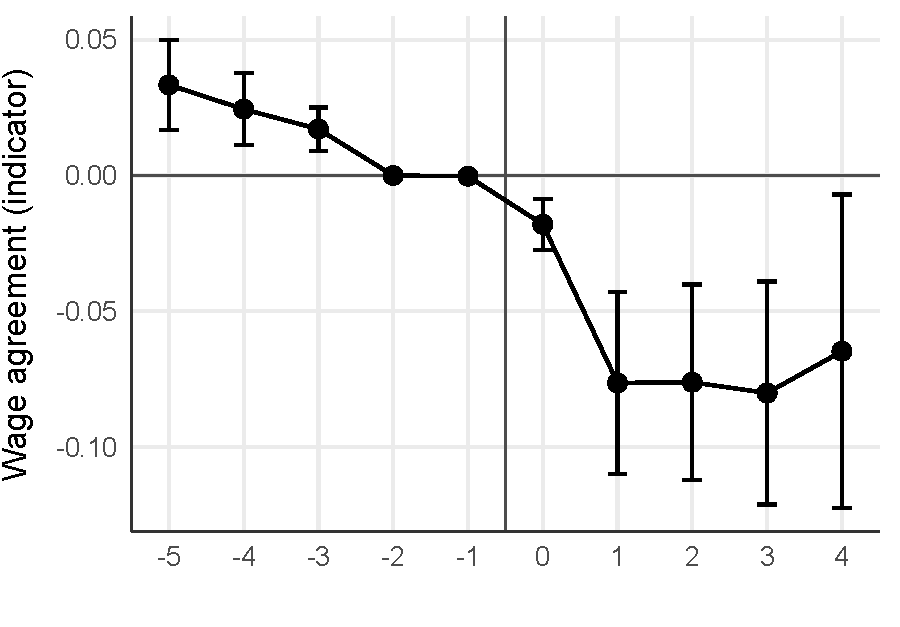
\includegraphics[width=\linewidth,max width=\linewidth]{figures/01_event_figures/figure_A21_a_wage_indicator.pdf}
	\end{subfigure}
	\begin{subfigure}[b]{.49\textwidth}
		\centering
		\caption[]{\small \# wage agreements (column~2)} \label{fig:nego:wage_num}
		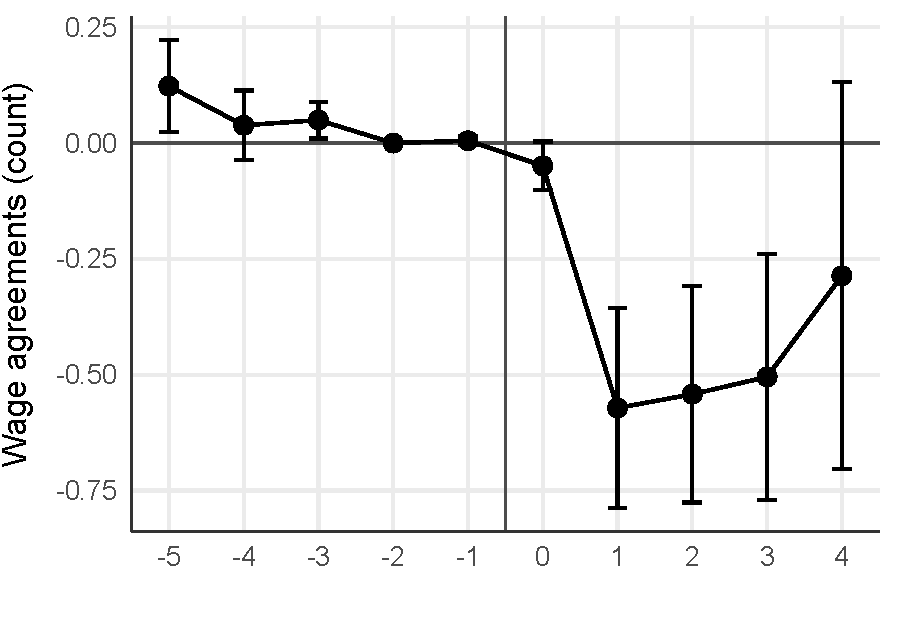
\includegraphics[width=\linewidth,max width=\linewidth]{figures/01_event_figures/figure_A21_b_wage_count.pdf}
	\end{subfigure}

	\begin{subfigure}[b]{.49\textwidth}
		\centering
		\caption[]{\small Hours agreement indicator (column~4)} \label{fig:nego:hours_ind}
		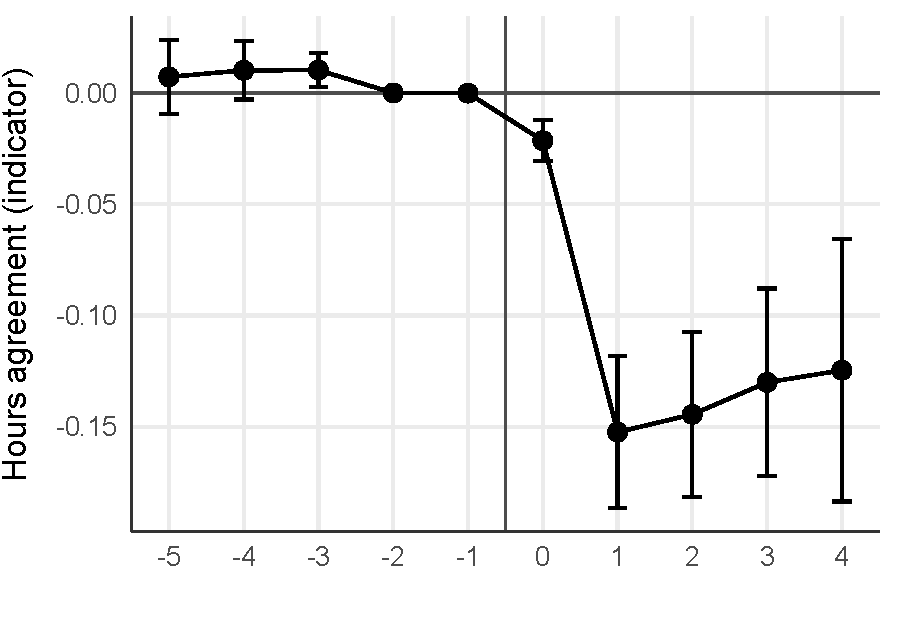
\includegraphics[width=\linewidth,max width=\linewidth]{figures/01_event_figures/figure_A21_c_hours_indicator.pdf}
	\end{subfigure}

	\floatfoot{{\footnotesize \textsc{Notes}: Event-study coefficients $\beta_d$ from equation~(\ref{eq:main_estimating_equation}) for three collective-agreement outcomes corresponding to columns~(1), (2) and~(4) of Table~\ref{tab:nego:LEnego_acc_result}. \textbf{Sample}: LE workers displaced after 2007 and their matched controls (the accords sub-sample); firm-level negotiation outcomes are measured over 2005--2007. \textbf{Specification}: baseline (no controls), reference period $d=-1$. Vertical bars denote 99\% confidence intervals based on robust standard errors clustered at the worker level.}}
\end{figure}


\begin{table}[h]
	\caption{Agreements robustness}	\label{tab:nego:LEnego_acc_rob}
	\begin{center}
{\footnotesize\begin{adjustbox}{max width=\linewidth}
\begin{tabular}{l|lllllll}\toprule
		% Generated from current results_analysis CSV files by master.R, section I (scripts/I-PLOTS_AND_TABLES).
% Table A19; status: ready
% Column 4 is acco_isin. Empty legacy lnsize coefficient row omitted because control coefficients are not exported.
% -- means a requested statistic is unavailable; an empty cell means not applicable.
 & (1) & (2) & (3) & (4) \\
Time to displ. & Wage agreement ind. & Wage agreement ind. & Wage agreement ind. & Wage agreement ind. \\
\midrule
$d=-3$ & 0.018 & 0.003 & 0.003 & 0.021 \\
 & (0.003) & (0.002) & (0.002) & (0.003) \\
$d=-2$ & REF & REF & REF & REF \\
 &  &  &  &  \\
$d=-1$ & -0.000 & -0.001 & -0.001 & -0.001 \\
 & (0.001) & (0.001) & (0.001) & (0.001) \\
$d=0$ & -0.014 & -0.010 & -0.011 & -0.023 \\
 & (0.004) & (0.003) & (0.003) & (0.004) \\
$d=1$ & -0.061 & -0.096 & -0.100 & -0.080 \\
 & (0.013) & (0.015) & (0.015) & (0.014) \\
$d=2$ & -0.059 & -0.088 & -0.092 & -0.083 \\
 & (0.014) & (0.017) & (0.016) & (0.015) \\
$d=3$ & -0.071 & -0.098 & -0.102 & -0.097 \\
 & (0.016) & (0.019) & (0.019) & (0.017) \\
$d=4$ & -0.059 & -0.063 & -0.070 & -0.081 \\
 & (0.022) & (0.028) & (0.028) & (0.023) \\
\midrule
Individuals & 28,198 & 28,198 & 28,198 & 27,650 \\
\# treated & 16,597 & 16,597 & 16,597 & 16,376 \\
Legal size bins (4) &  &  & $\surd$ &  \\

		\bottomrule
\end{tabular}
\end{adjustbox}}			
		%\input{03_Draft/tables/LEnego_acc_rob.tex}  
		\floatfoot{{\footnotesize \textsc{Notes}: This table presents event-study estimates of the reallocation of workers displaced for economic reason (LE) across firms with different approach to collective agreement ---see equation (\ref{eq:main_estimating_equation}) and associated text for more details on the specification. \textbf{Comment on timing}: Firm-level outcomes are computed over the 2005-2007 period. To limit the risk of reverse causality we restrict our sample to individuals displaced after 2007. We thus do not observe individuals after $t^D+4$. Accordingly, event-study coefficients reflect the movement of displaced workers to firms with different initial characteristics and \textit{not} changes within-firm in such characteristics. \textbf{Specification}: Column (1) replicates the first column of Table \ref{tab:nego:LEnego_acc_result}. Column (2) adds a control for the logarithm of employers' number of employee to our main equation. Column (3) further adds a fixed effect for four size categories (from 0 to 10, from 11 to 49, from 50 to 299 and above 299 employees). Finally column (4) transforms the outcome of interest by ignoring those firms that are never observed in the agreement database. \textbf{Outcomes}: Table \ref{apptab:definitions} summarizes variables' definition. Wage agreement indicator is an indicator taking value 1 if the firm has signed (at least) one agreement relative to wages over the period. Details are given in \ref{appsec:accord_data}. \textbf{Standard errors}: robust standard errors clustered at the worker-level.}}
	\end{center}
\end{table}


\begin{table}[h] 
\caption{Election results} \label{tab:nego:LEnego_ele_result}
\begin{center}
{\footnotesize\begin{adjustbox}{max width=\linewidth}
\begin{tabular}{l|lll}\toprule
	% Generated from current results_analysis CSV files by master.R, section I (scripts/I-PLOTS_AND_TABLES).
% Table A20; status: ready
% Failed elections follow the paper definition: shinscrit_carence_siren0912.
% -- means a requested statistic is unavailable; an empty cell means not applicable.
 & (1) & (2) & (3) \\
Time to displ. & Average turnout & Failed (\% workers) & CGT (\% workers) \\
\midrule
$d=-3$ & -0.007 & -0.002 & 0.003 \\
 & (0.001) & (0.001) & (0.002) \\
$d=-2$ & REF & REF & REF \\
 &  &  &  \\
$d=-1$ & 0.000 & 0.000 & -0.000 \\
 & (0.000) & (0.000) & (0.000) \\
$d=0$ & -0.018 & -0.000 & 0.009 \\
 & (0.002) & (0.002) & (0.002) \\
$d=1$ & -0.170 & 0.002 & 0.093 \\
 & (0.010) & (0.009) & (0.012) \\
$d=2$ & -0.139 & 0.017 & 0.067 \\
 & (0.010) & (0.010) & (0.013) \\
$d=3$ & -0.115 & 0.019 & 0.052 \\
 & (0.010) & (0.010) & (0.013) \\
$d=4$ & -0.097 & 0.032 & 0.045 \\
 & (0.011) & (0.011) & (0.014) \\
$d=5$ & -0.089 & 0.036 & 0.040 \\
 & (0.012) & (0.012) & (0.015) \\
$d=6$ & -0.088 & 0.043 & 0.044 \\
 & (0.013) & (0.013) & (0.017) \\
\midrule
Individuals & 29,971 & 29,971 & 29,971 \\
\# treated & 17,071 & 17,071 & 17,071 \\
 
	\bottomrule
\end{tabular}
\end{adjustbox}}	
\floatfoot{{\footnotesize \textsc{Notes}: This table presents event-study estimates of the reallocation of workers displaced for economic reason (LE) across firms with different professional election turnout ---see equation (\ref{eq:main_estimating_equation}) and associated text for more details on the specification. \textbf{Comment on timing}: Firm-level outcomes are computed over the 2009-2012 period. Because of a risk of reverse causality, we perform robustness checks in Table \ref{tab:nego:LEnego_ele_rob}. Because we fix firm-characteristics over time, event-study coefficients reflect the movement of displaced workers to firms with different initial characteristics and \textit{not} changes within-firm in such characteristics. \textbf{Outcomes}: Table \ref{apptab:definitions} summarizes variables' definition. Average turnout is at elections held by the firm between 2009-2012 (worker-weighted). Failed is share of workers covered by a failed election. CGT is the share of workers covered by a (potential) CGT DS representative. Details are given in \ref{appsec:elec_data}. \textbf{Standard errors}: robust standard errors clustered at the worker-level.}}
\end{center}
\end{table}

\begin{table}[h] 
\caption{Election robustness}\label{tab:nego:LEnego_ele_rob}
\begin{center}
{\footnotesize\begin{adjustbox}{max width=\linewidth}
\begin{tabular}{l|lll}\toprule
		% Generated from current results_analysis CSV files by master.R, section I (scripts/I-PLOTS_AND_TABLES).
% Table A21; status: ready
% Column 3: log size + legal size bins. Column 4: sample: lowest quartile of layoff share, at cutoff0.00671140939597315
% -- means a requested statistic is unavailable; an empty cell means not applicable.
 & (1) & (2) & (3) & (4) \\
Time to displ. & Average turnout & Average turnout & Average turnout & Average turnout \\
\midrule
$d=-3$ & -0.007 & -0.006 & -0.005 & -0.002 \\
 & (0.001) & (0.001) & (0.001) & (0.001) \\
$d=-2$ & REF & REF & REF & REF \\
 &  &  &  &  \\
$d=-1$ & 0.000 & 0.000 & 0.000 & 0.000 \\
 & (0.000) & (0.000) & (0.000) & (0.000) \\
$d=0$ & -0.018 & -0.017 & -0.016 & -0.009 \\
 & (0.002) & (0.002) & (0.002) & (0.002) \\
$d=1$ & -0.165 & -0.158 & -0.152 & -0.202 \\
 & (0.010) & (0.009) & (0.009) & (0.013) \\
$d=2$ & -0.136 & -0.130 & -0.125 & -0.165 \\
 & (0.010) & (0.010) & (0.010) & (0.014) \\
$d=3$ & -0.112 & -0.108 & -0.105 & -0.142 \\
 & (0.010) & (0.010) & (0.010) & (0.016) \\
$d=4$ & -0.095 & -0.090 & -0.087 & -0.113 \\
 & (0.011) & (0.011) & (0.011) & (0.017) \\
$d=5$ & -0.086 & -0.082 & -0.080 & -0.103 \\
 & (0.012) & (0.012) & (0.012) & (0.019) \\
$d=6$ & -0.084 & -0.080 & -0.078 & -0.111 \\
 & (0.013) & (0.013) & (0.013) & (0.022) \\
\midrule
Individuals & 29,971 & 29,971 & 29,971 & 7,953 \\
\# treated & 17,071 & 17,071 & 17,071 & 4,144 \\
Legal size bins (4) &  &  & $\surd$ &  \\

		\bottomrule
\end{tabular}
\end{adjustbox}}
%\scalebox{.8}{\input{03_Draft/tables/LEnego_ele_rob.tex}}
\floatfoot{{\footnotesize \textsc{Notes}: This table presents event-study estimates of the reallocation of workers displaced for economic reason (LE) across firms with different professional election turnout ---see equation (\ref{eq:main_estimating_equation}) and associated text for more details on the specification. \textbf{Comment on timing}: Firm-level outcomes are computed over the 2009-2012 period. We perform robustness checks in this table. Because we fix firm-characteristics over time, event-study coefficients reflect the movement of displaced workers to firms with different initial characteristics and \textit{not} changes within-firm in such characteristics. \textbf{Outcomes}: Table \ref{apptab:definitions} summarizes variables' definition. Average turnout is at elections held by the firm between 2009-2012 (worker-weighted). Details are given in \ref{appsec:elec_data}. \textbf{Specifications}: Column (1) replicates the first column of Table \ref{tab:nego:LEnego_ele_result}. Column (2) replicates column (1) but controlling for firm size. Column (3) estimates the effect on a sub-sample made of the quarter of laid-off workers that were part of the smallest layoff (as a share of firm employment). \textbf{Standard errors}: robust standard errors clustered at the worker-level.}}
\end{center}
\end{table}
